% !TeX program = xelatex
\documentclass[11pt,a4paper]{article}

\usepackage{fontspec}
\usepackage{ucharclasses}
\usepackage{amsmath,amssymb,mathtools}
\usepackage{geometry}
\usepackage{setspace}
\usepackage{xcolor}
\usepackage{booktabs,longtable,tabularx,array}
\usepackage{enumitem}
\usepackage{titlesec}
\usepackage{fancyhdr,lastpage}
\usepackage{caption}
\usepackage{float}
\usepackage{graphicx}
\usepackage{tcolorbox}
\tcbuselibrary{breakable,skins}
\usepackage{xurl}
\usepackage{hyperref}

\defaultfontfeatures{Ligatures=TeX}
\setmainfont{NotoSerifSC-Regular.ttf}[
  Path=fonts/,
  BoldFont=NotoSerifSC-Bold.ttf,
  ItalicFont=NotoSerifSC-Regular.ttf,
  BoldItalicFont=NotoSerifSC-Bold.ttf,
  ItalicFeatures={FakeSlant=0.16},
  BoldItalicFeatures={FakeSlant=0.16}
]
\setsansfont{NotoSansSC-Regular.ttf}[
  Path=fonts/,
  BoldFont=NotoSansSC-Bold.ttf
]
\setmonofont{Latin Modern Mono}
\newfontfamily\latinserif{NimbusRoman-Regular.otf}[
  Path=fonts/,
  BoldFont=NimbusRoman-Bold.otf,
  ItalicFont=NimbusRoman-Italic.otf,
  BoldItalicFont=NimbusRoman-BoldItalic.otf
]
\newfontfamily\latinsans{NimbusSans-Regular.otf}[
  Path=fonts/,
  BoldFont=NimbusSans-Bold.otf,
  ItalicFont=NimbusSans-Italic.otf,
  BoldItalicFont=NimbusSans-BoldItalic.otf
]
\newfontfamily\cnserif{NotoSerifSC-Regular.ttf}[
  Path=fonts/,
  BoldFont=NotoSerifSC-Bold.ttf,
  ItalicFont=NotoSerifSC-Regular.ttf,
  BoldItalicFont=NotoSerifSC-Bold.ttf,
  ItalicFeatures={FakeSlant=0.16},
  BoldItalicFeatures={FakeSlant=0.16}
]
\newfontfamily\cnsans{NotoSansSC-Regular.ttf}[
  Path=fonts/,
  BoldFont=NotoSansSC-Bold.ttf
]
\setTransitionsForLatin{\latinserif}{\cnserif}
\newcommand{\headingfonts}{%
  \cnsans
  \setTransitionsForLatin{\latinsans}{\cnsans}%
  \cnsans
}
\XeTeXlinebreaklocale "zh"
\XeTeXlinebreakskip=0pt plus 1pt

\geometry{left=2.2cm,right=2.2cm,top=2.2cm,bottom=2.2cm,headheight=15pt}
\setstretch{1.55}
\setlength{\parindent}{2em}
\setlength{\parskip}{0pt}
\setlength{\emergencystretch}{2em}
\renewcommand{\arraystretch}{1.18}
\setlist{nosep,leftmargin=2em}
\setlist[itemize]{label=$\bullet$}

\definecolor{DeepBlue}{HTML}{17365D}
\definecolor{MainBlue}{HTML}{1D4E89}
\definecolor{SoftBlue}{HTML}{EEF5FC}
\definecolor{SoftGray}{HTML}{F4F5F7}
\definecolor{RuleGray}{HTML}{BFC7D1}
\definecolor{GainGreen}{HTML}{2F7D4A}
\definecolor{WarnRed}{HTML}{A33A3A}

\titleformat{\section}
  {\headingfonts\Large\bfseries\color{DeepBlue}}
  {\thesection}{0.7em}{}
\titleformat{\subsection}
  {\headingfonts\large\bfseries\color{MainBlue}}
  {\thesubsection}{0.7em}{}
\titleformat{\subsubsection}
  {\headingfonts\normalsize\bfseries}
  {\thesubsubsection}{0.6em}{}
\titlespacing*{\section}{0pt}{1.35em}{0.50em}
\titlespacing*{\subsection}{0pt}{1.05em}{0.35em}

\pagestyle{fancy}
\fancyhf{}
\fancyhead[L]{\small SMPR 完整实验与可靠性报告}
\fancyhead[R]{\small Frozen V5/V6/V7 Evidence}
\fancyfoot[C]{\small \thepage/\pageref{LastPage}}
\renewcommand{\headrulewidth}{0.4pt}

\renewcommand{\figurename}{图}
\renewcommand{\tablename}{表}
\renewcommand{\contentsname}{目\quad 录}
\captionsetup{
  font={small,bf},
  labelfont=bf,
  labelsep=quad,
  justification=centering,
  singlelinecheck=false
}

\hypersetup{
  colorlinks=true,
  linkcolor=DeepBlue,
  urlcolor=MainBlue,
  pdftitle={SMPR 冻结实验、公开复现与外部验证结果报告},
  pdfauthor={Anonymous Author},
  pdfsubject={Qubit-routing experiment, reliability audit and reproducibility},
  pdfkeywords={SMPR, LightSABRE, qubit routing, blind test, reliability audit}
}

\newtcolorbox{summarybox}[1][]{
  breakable,
  enhanced,
  colback=SoftBlue,
  colframe=MainBlue,
  boxrule=0.7pt,
  arc=1.2mm,
  left=2.5mm,right=2.5mm,top=1.8mm,bottom=1.8mm,
  #1
}
\newtcolorbox{notebox}[1][]{
  breakable,
  enhanced,
  colback=SoftGray,
  colframe=RuleGray,
  boxrule=0.6pt,
  arc=1.2mm,
  left=2.5mm,right=2.5mm,top=1.8mm,bottom=1.8mm,
  #1
}
\newcolumntype{Y}{>{\raggedright\arraybackslash}X}
\newcolumntype{C}[1]{>{\centering\arraybackslash}p{#1}}

\begin{document}

\begin{center}
  {\headingfonts\fontsize{21}{29}\selectfont\bfseries
  SMPR 冻结实验、公开复现与外部验证结果报告\par}
  \vspace{0.45em}
  {\latinsans\large\bfseries
  Frozen Experiment, Reliability Audit and Reproduction Report\par}
  \vspace{1.1em}
  {\large Anonymous Author\par}
  \vspace{0.3em}
  {\small 公开核心：1.0.0-rc3\quad 证据日期：2026-07-25\quad 报告状态：V5/V6/V7 已复核\par}
\end{center}

\vspace{0.8em}

\begin{summarybox}
\textbf{执行摘要。}
本报告对安全多布局组合路由器 SMPR 的冻结 V5/V6 证据进行独立整理、逐项复算与
发布复核。V6 的 120 个预注册盲测实例上，20-seed LightSABRE 共需 3176 个
SWAP，SMPR 共需 3051 个，减少 125 个（3.9358\%）；逐实例 SWAP 胜/平/负为
50/70/0。实例级与因子单元级 bootstrap 的 95\% 区间分别为
$[-0.024346,-0.013634]$ 与 $[-0.024392,-0.013594]$，上端均低于零。
语义、拓扑和指标审计全部通过。2026-07-25 的独立环境完整重跑再次得到相同
V5/V6 质量总量与零主质量差异，并对证据包及其 18 个内部文件逐一通过 SHA-256
校验。随后按结果不可见条件下冻结的 V7 规程执行 10 条 QASMBench 公共线路、
11--23 逻辑比特和 19/57 比特 heavy-hex 的三次同机重复，共得到 120 条
质量--时间观测。SMPR 在 LightSABRE 的 $0.25T,0.5T,T,2T$ 四档预算下
分别减少 11.05\%、8.84\%、7.30\% 和 5.17\% 的总 SWAP；四个线路聚类
95\% 区间均轻微跨零，因此报告总量优势及其趋势，但不宣称 95\% 水平下显著。
V7 的冻结、环境、结果哈希和三项 120/120 审计全部通过。
\end{summarybox}

\tableofcontents
\newpage

\section{报告目标与结论边界}

\subsection{目标}

本报告面向论文评审、答辩复核和第三方复现，回答五个问题：

\begin{enumerate}
  \item 冻结参数下，SMPR 是否在 V6 盲测上降低总 SWAP；
  \item 候选组合是否保持逐实例 LightSABRE 质量下界；
  \item 统计结论是否对因子单元相关性与留一层级检查稳定；
  \item 代码、环境、输出和哈希证据能否形成可追踪的复现链；
  \item 在公共线路、超过 10 比特和 heavy-hex 上，同机质量--时间关系是否仍有利于 SMPR。
\end{enumerate}

\subsection{可支持与不可支持的表述}

\begin{table}[H]
\centering
\caption{证据所支持的结论边界}
\begin{tabularx}{\textwidth}{C{1.7cm}Y}
\toprule
状态 & 表述 \\
\midrule
\textcolor{GainGreen}{可支持}
& 冻结 V6 的 120 个实例上，SMPR 相对 20-seed LightSABRE 减少
3.9358\% 总 SWAP，逐实例无 SWAP 退化。\\
\textcolor{GainGreen}{可支持}
& 实例级和因子单元级 bootstrap 区间均完全低于零；所有留一层级后的总改善仍为正。\\
\textcolor{GainGreen}{可支持}
& V5/V6 全部实例通过语义、拓扑和指标审计；独立环境重跑得到相同质量总量。\\
\textcolor{GainGreen}{可支持}
& V7 四档同机匹配预算的总 SWAP 均低于 LightSABRE，且冻结、环境、哈希、
路由轨迹、拓扑和内部质量下界审计全部通过。\\
\textcolor{WarnRed}{不可支持}
& SMPR 在任意拓扑与线路上都保证严格改善，或任一内部展开分支普遍优于 LightSABRE。\\
\textcolor{WarnRed}{不可支持}
& V7 已在 95\% 水平证明 SMPR 普遍优于时间匹配 LightSABRE；四个线路聚类区间均包含零。\\
\textcolor{WarnRed}{不可支持}
& 当前公共线路和 11--23 比特结果已经代表全部真实硬件、方向约束和误差率条件。\\
\bottomrule
\end{tabularx}
\end{table}

\section{证据层级与冻结过程}

\subsection{证据层级}

本项目将证据分为四层。第一层是 V6 预注册盲测，承担主要质量推断；第二层是
V5 工程复核，验证冻结等价、执行器一致性和软件回归；第三层是独立公开环境
重跑，验证发布包可执行性与数值一致性；第四层是结果不可见条件下冻结的 V7
公共线路外部验证，用于检验规模、拓扑和质量--时间关系的可迁移性。V7 不改变
V6 的确认性地位，其区间跨零结果按探索性外部证据报告。

\begin{table}[H]
\centering
\caption{数据与证据角色}
\begin{tabularx}{\textwidth}{C{1.4cm}C{1.5cm}Y Y}
\toprule
数据 & 实例 & 主要用途 & 推断地位 \\
\midrule
V5 & 60 & 参数冻结、实现等价、执行器与发布复核 & 工程证据，不作为独立确认性样本 \\
V6 & 120 & 冻结后生成的两实现因子设计盲测 & 主要确认性证据 \\
重跑 & 180 & 新环境完整执行 V5、V6 与联合统计审计 & 可执行性与质量一致性证据 \\
V7 & 10 条线路、120 条观测 & 公共线路、heavy-hex、超过 10 比特与同机质量--时间 & 前瞻冻结的探索性外部证据 \\
\bottomrule
\end{tabularx}
\end{table}

\subsection{冻结顺序}

\begin{enumerate}
  \item 仅使用开发数据固定候选组合与选择参数；
  \item 固定 V6 清单、生成规则、种子派生与主要统计规则；
  \item 生成并执行 V6，在结果不可见的条件下完成主要分析；
  \item 按预注册规则计算实例级 bootstrap；
  \item 只改进持久分片执行和证据汇总，不改变质量候选；
  \item 增补因子单元 bootstrap、留一层级与逐实例审计，并明确标注为事后稳健性分析；
  \item 在隔离环境中独立重跑，整理公开名称、修正依赖并形成发布归档；
  \item 在结果不可见时冻结 V7 的 82 个文件，完成三次同机重复并独立复算分析。
\end{enumerate}

\begin{notebox}
因子单元 cluster bootstrap 是事后稳健性分析，不能追溯标记为预注册分析。
公开整理和独立重跑没有依据 V6 结果重新选择参数。
\end{notebox}

\section{方法与冻结配置}

\subsection{比较对象}

\begin{table}[H]
\centering
\caption{候选与最终选择的实验角色}
\begin{tabularx}{\textwidth}{C{3.2cm}Y}
\toprule
名称 & 定义 \\
\midrule
LightSABRE & Qiskit SABRE 自动布局和路由；20 个种子中按质量取优，作为显式质量下界。\\
独立展开分支 & 从自身布局池执行完整基线策略展开，用于衡量独立候选的互补性。\\
双分支选择 & 在 LightSABRE 与独立展开分支之间取优，用于分解跨布局带来的新增收益。\\
跨布局分支 & 从 LightSABRE 并列最优布局及其一换位邻域冷启动完整路由。\\
SMPR & 对所有真实候选按固定质量键统一选择，并对结果执行三重审计。\\
\bottomrule
\end{tabularx}
\end{table}

每个候选首先比较 SWAP 数，再比较加权深度。SWAP 在加权深度中按三个 CX
计入，其他一、双比特门权重为一。主要配对统计量为

\[
\bar{\Delta}=
\frac{1}{N}\sum_{i=1}^{N}
\frac{S_i^{\mathrm{SMPR}}-S_i^{\mathrm{LS}}}{M_i},
\]

其中 $M_i$ 为输入 CX 数；$\bar{\Delta}<0$ 有利于 SMPR。

\subsection{冻结参数}

\begin{table}[H]
\centering
\caption{冻结实验参数}
\begin{tabularx}{\textwidth}{Y Y C{3.0cm}}
\toprule
模块 & 参数 & 值 \\
\midrule
LightSABRE & 种子数 $\times$ 重复 & $20\times1$ \\
有序势函数 & 扩展衰减 & $2^{-i}$ \\
一步代理 & $(\beta,\rho,\alpha)$ & $(2.0,0,0.5)$ \\
完整展开 & 候选宽度 & 通常 2；特定情形为 4 \\
跨布局 & 基布局 & 全部并列最优唯一布局 \\
跨布局 & 每布局邻域数 & 4 \\
布局代理 & 衰减 $\gamma$ & 0.95 \\
最终选择 & 主质量键 & (SWAP，加权深度) \\
持久执行 & 分片数与调度 & 4 / LPT \\
统计 & 次数与种子 & 10000 / 20260723 \\
\bottomrule
\end{tabularx}
\end{table}

\section{数据设计}

V5 与 V6 使用相同的因子空间：四种硬件拓扑（line、ring、grid、random）、
五种线路模式（uniform、far、phase\_shift、alternating、
parallel\_layers）、量子比特数 6、8、10，以及长度因子 3、6、12。
输入 CX 数满足 $M=n\times f$。线路门集为 H 和 CX。

V5 对每个“拓扑 $\times$ 模式 $\times$ 长度因子”单元给出一个实现，共
$4\times5\times3=60$ 例。V6 对每个单元给出两个独立实现，共 120 例。
量子比特数通过固定规则在单元间平衡。因此 V6 的 60 个因子单元都恰含两个
实现，允许在实例级分析之外执行单元级重采样。

\begin{table}[H]
\centering
\caption{V6 平衡性}
\begin{tabular}{lrr}
\toprule
分组 & 层级数 & 每层实例 \\
\midrule
拓扑 & 4 & 30 \\
线路模式 & 5 & 24 \\
量子比特数 & 3 & 40 \\
长度因子 & 3 & 40 \\
因子单元 & 60 & 2 \\
\bottomrule
\end{tabular}
\end{table}

\section{运行环境与完整复现过程}

\subsection{冻结软件环境}

\begin{table}[H]
\centering
\caption{2026-07-25 独立环境记录}
\begin{tabularx}{\textwidth}{C{4.2cm}Y}
\toprule
项目 & 记录 \\
\midrule
操作系统 & Windows \\
Python & 3.10.11 \\
Qiskit & 2.4.2 \\
OpenQASM 3 导入器 & qiskit-qasm3-import 0.6.0 \\
哈希种子 & PYTHONHASHSEED=0 \\
执行器 & 4 个持久分片，LPT 调度 \\
软件版本 & SMPR public-core 1.0.0-rc3；冻结质量逻辑与证据复现包兼容 \\
\bottomrule
\end{tabularx}
\end{table}

\subsection{复现步骤}

完整过程按以下顺序执行：

\begin{enumerate}
  \item 验证源发布清单、数据集哈希、依赖版本与核心模块依赖闭包；
  \item 运行公开核心的静态检查、20 项 Python 内置测试以及冻结环境集成测试；
  \item 运行五例 V5 冒烟测试，确认 OpenQASM 3 往返审计可用；
  \item 完整运行 V5，采用严格逐字段质量策略；
  \item 完整运行 V6，采用主质量字段策略；
  \item 对新生成的 V5/V6 结果执行联合可靠性审计；
  \item 整理控制台记录、环境记录、逐实例表、摘要和哈希清单；
  \item 对证据 ZIP 和内部 18 个文件重新计算 SHA-256；
  \item 从原始冻结字段生成不含本机绝对线路路径的对外逐实例表；
  \item 准备并冻结 V7，连续完成三次同机质量--时间实验；
  \item 复核 V7 的 120 条观测、嵌套哈希和独立分析重算。
\end{enumerate}

V6 的主质量字段策略仍检查最终来源、SWAP、深度和三项审计。它仅排除已经由
独立单例复跑确认的一个未选中辅助候选深度差异。该差异没有改变最终来源、
最终质量或审计结果。

\section{总体结果}

\begin{table}[H]
\centering
\caption{完整质量总量}
\begin{tabular}{lrrrrrr}
\toprule
数据 & 实例 & LightSABRE & 独立展开 & 双分支 & SMPR & 改善 \\
\midrule
V5 & 60 & 1691 & 1843 & 1670 & 1641 & 50（2.9568\%）\\
V6 & 120 & 3176 & 3386 & 3119 & 3051 & 125（3.9358\%）\\
\bottomrule
\end{tabular}
\end{table}

V6 上，双分支选择相对 LightSABRE 减少 57 个 SWAP；跨布局分支加入后再
减少 68 个。因此，最终 125 个改善中的 54.4\% 是跨布局分支相对双分支选择
带来的新增收益。最终来源为 LightSABRE 62 例、跨布局分支 51 例、独立展开
分支 7 例。这种来源分布说明 SMPR 是互补候选的组合，而不是由单一分支替代
强基线。

\begin{figure}[H]
\centering
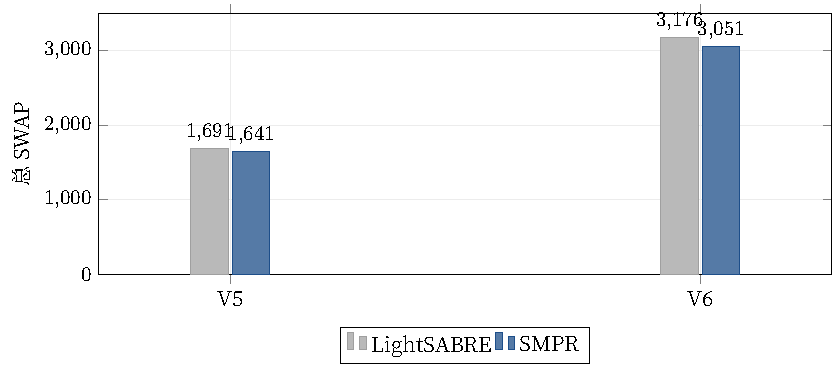
\includegraphics[width=0.88\textwidth]{figures/fig_v5_v6_totals.pdf}
\caption{V5/V6 总 SWAP 对比}
\end{figure}

\section{逐实例统计推断}

\subsection{预注册实例级分析}

\begin{table}[H]
\centering
\caption{V6 逐实例主要统计量}
\begin{tabular}{lr}
\toprule
指标 & 结果 \\
\midrule
SWAP 胜/平/负 & 50/70/0 \\
质量胜/平/负 & 58/62/0 \\
平均绝对 SWAP 改善 & 1.041667 \\
中位绝对改善 & 0 \\
最大单例改善 & 11 \\
平均归一化配对差值 & $-0.018726852$ \\
实例级 bootstrap 95\% 区间 & $[-0.024346,-0.013634]$ \\
\bottomrule
\end{tabular}
\end{table}

预注册分析使用固定种子 20260723 进行 10,000 次有放回实例级 percentile
bootstrap。区间上端小于零，预注册判据通过。中位改善为零是因为 70/120
实例在 SWAP 上平局；因此总量、胜平负和区间必须一起报告，不能只给出平均
百分比。

\subsection{因子单元稳健性}

补充稳健性分析以 60 个“拓扑 $\times$ 模式 $\times$ 长度因子”单元为抽样单位。
每次抽中一个单元时同时保留其中两个实现。10,000 次 cluster bootstrap 得到

\[
[-0.024392,\,-0.013594].
\]

该区间与实例级结果接近并完全低于零，表明主要结论对单元内相关性的处理不
敏感。它是事后稳健性分析，而非预注册结果。

\subsection{留一层级检查}

分别删除一种拓扑、一种线路模式或一个长度因子后，剩余实例的总 SWAP 改善率
均为正，范围为 3.2090\%--4.5513\%。因此总体收益没有完全依赖某个单独层级；
但该检查仍不能替代新分布上的外部验证。

\section{分组结果}

\subsection{拓扑与线路模式}

\begin{table}[H]
\centering
\caption{V6 按拓扑分组}
\begin{tabular}{lrrrrr}
\toprule
拓扑 & 实例 & LightSABRE & SMPR & 改善率 & 胜/平/负 \\
\midrule
grid & 30 & 524 & 515 & 1.72\% & 7/23/0 \\
line & 30 & 1321 & 1270 & 3.86\% & 16/14/0 \\
random & 30 & 461 & 447 & 3.04\% & 10/20/0 \\
ring & 30 & 870 & 819 & 5.86\% & 17/13/0 \\
\bottomrule
\end{tabular}
\end{table}

\begin{table}[H]
\centering
\caption{V6 按线路模式分组}
\begin{tabular}{lrrrrr}
\toprule
模式 & 实例 & LightSABRE & SMPR & 改善率 & 胜/平/负 \\
\midrule
alternating & 24 & 620 & 594 & 4.19\% & 12/12/0 \\
far & 24 & 450 & 429 & 4.67\% & 10/14/0 \\
parallel\_layers & 24 & 847 & 828 & 2.24\% & 6/18/0 \\
phase\_shift & 24 & 486 & 471 & 3.09\% & 9/15/0 \\
uniform & 24 & 773 & 729 & 5.69\% & 13/11/0 \\
\bottomrule
\end{tabular}
\end{table}

ring 的总改善率最高，grid 最低；uniform 的改善率最高，
parallel\_layers 最低。所有分组的胜/平/负均没有负例。分组差异用于描述
候选互补性，不应被解释为经过独立检验的因果结论。

\subsection{量子比特数与长度因子}

\begin{table}[H]
\centering
\caption{V6 按量子比特数分组}
\begin{tabular}{lrrrrr}
\toprule
量子比特 & 实例 & LightSABRE & SMPR & 改善 & 改善率 \\
\midrule
6 & 40 & 489 & 433 & 56 & 11.45\% \\
8 & 40 & 1125 & 1087 & 38 & 3.38\% \\
10 & 40 & 1562 & 1531 & 31 & 1.98\% \\
\bottomrule
\end{tabular}
\end{table}

\begin{table}[H]
\centering
\caption{V6 按长度因子分组}
\begin{tabular}{lrrrrr}
\toprule
长度因子 & 实例 & LightSABRE & SMPR & 改善 & 改善率 \\
\midrule
3 & 40 & 392 & 378 & 14 & 3.57\% \\
6 & 40 & 858 & 823 & 35 & 4.08\% \\
12 & 40 & 1926 & 1850 & 76 & 3.95\% \\
\bottomrule
\end{tabular}
\end{table}

量子比特数增大时改善率下降。一个合理但尚未单独验证的机制是：每个基布局只
保留四个邻域，固定预算随布局空间增长而覆盖更小比例。长度分组的改善率较
接近，说明收益并不只来自最长线路。

\section{正确性与执行一致性}

\subsection{三重审计}

\begin{table}[H]
\centering
\caption{冻结结果的正确性检查}
\begin{tabularx}{\textwidth}{Y C{1.5cm} C{1.5cm} Y}
\toprule
审计 & V5 & V6 & 判据 \\
\midrule
语义等价 & 60/60 & 120/120 & Clifford 表示与期望物理线路完全相等 \\
拓扑合法 & 60/60 & 120/120 & 每个双比特门位于耦合边 \\
指标一致 & 60/60 & 120/120 & 重算 SWAP、CX 和深度与记录一致 \\
映射合法 & 60/60 & 120/120 & 初始和最终映射都是单射 \\
质量下界 & 60/60 & 120/120 & SMPR 不劣于 20-seed LightSABRE \\
\bottomrule
\end{tabularx}
\end{table}

当前线路只含 Clifford 门，因此 Clifford 表示给出精确的语义比较。若扩展到
非 Clifford 门集，需要增加适用于通用线路的等价检查，不能直接沿用当前审计
覆盖声明。

\subsection{辅助字段差异}

持久执行与冻结 V6 结果比较时，主质量字段差异为零，辅助字段差异
为一。差异位于第 39 例未选中独立展开候选的深度：旧参考为 29，持久运行与
独立单例重跑均为 27。最终来源仍为跨布局分支，最终质量仍为 7 个 SWAP、
加权深度 28，三项审计均通过。最终复现因而保留原冻结证据，并在 V6 复现时
采用主质量字段策略，避免把未选中候选的辅助深度误当成最终质量退化。

\section{执行性能与工程可靠性}

\subsection{冻结执行器比较}

\begin{table}[H]
\centering
\caption{旧执行方式与持久分片执行比较}
\begin{tabular}{lrrrr}
\toprule
数据 & 旧墙钟 & 持久分片 & 加速比 & 墙钟降幅 \\
\midrule
V5 & 212.569 s & 78.975 s & 2.692$\times$ & 62.85\% \\
V6 & 583.840 s & 200.207 s & 2.916$\times$ & 65.71\% \\
\bottomrule
\end{tabular}
\end{table}

该比较只说明持久分片减少重复进程启动并提高同一 SMPR 组合流程的执行效率。
它不是 SMPR 与单独 LightSABRE 的端到端时间比较。

\subsection{2026-07-25 独立重跑}

\begin{table}[H]
\centering
\caption{公开候选包在隔离环境中的完整重跑}
\begin{tabular}{lrrrrrr}
\toprule
数据 & 实例 & LightSABRE & SMPR & 减少 & 墙钟 & 质量差异 \\
\midrule
V5 & 60 & 1691 & 1641 & 50 & 195.156 s & 0 \\
V6 & 120 & 3176 & 3051 & 125 & 527.188 s & 0 \\
\bottomrule
\end{tabular}
\end{table}

V5/V6 本次没有使用逐例实测计时参考，且机器、解释器与后台负载记录不同，
因此 195.156\,s 和 527.188\,s 只证明公开候选包可完整执行，不替换原执行器
比较。新重跑分别避免 56 和 116 次进程重启，三项审计均全数通过。

\subsection{软件检查}

公开核心的自动检查覆盖：

\begin{itemize}
  \item 核心路由状态、映射合法性、最短路径缓存与基线等价；
  \item 确定性选择键、并列最优布局去重和旧证据兼容选择；
  \item 持久分片恢复、配置不一致拒绝和质量策略；
  \item 联合统计审计与冻结证据复算；
  \item 包版本、数据集哈希、模块闭包、Qiskit 与 OpenQASM 3 依赖；
  \item 旧内部名称、敏感凭据文件名与未入清单文件的发布前检查。
\end{itemize}

公开核心当前包含 20 项模型、配置、事务式准备和发布结构测试；冻结环境还需
运行 Qiskit 集成测试、五例冒烟测试与 V5/V6 全量参考相等性。输出目录默认
拒绝覆盖；恢复模式只接受完整且配置一致的分片，避免旧结果静默混入新实验。

\subsection{公开核心与研发过程复现包}

发布物采用双包结构。公开核心只含运行 SMPR 所需的 29 模块依赖闭包、冻结
V5/V6 输入与参考表、统一 CLI、测试、V7 规程和发布校验；模块以
\texttt{routing\_model}、\texttt{rollout\_policy}、
\texttt{layout\_proxy}、\texttt{smpr\_portfolio} 等职责命名，文本检查
发现旧内部算法名或编号开发脚本名即失败。完整研发过程则原样保留 1--64 的
开发脚本、旧字段、早期数据、运行记录和结果，只承担证据追踪，不作为公共 API。

\begin{table}[H]
\centering
\caption{双包发布治理}
\begin{tabularx}{\textwidth}{p{0.25\textwidth}p{0.29\textwidth}Y}
\toprule
交付物 & 面向对象 & 内容与约束 \\
\midrule
SMPR 公开核心 &
使用者、评审者、后续开发者 &
描述性模块、统一命令行、冻结参考、V7、测试和源清单；不含旧内部名称。\\
完整研发复现包 &
复现审计者、项目作者 &
原样研发过程、旧字段、运行记录和逐文件 SHA-256；不保证稳定接口。\\
正式论文包 &
投稿与答辩 &
主论文、完整实验报告、参考文献、V5/V6 证据表和 V7 质量--时间结果。\\
\bottomrule
\end{tabularx}
\end{table}

公开核心当前使用严格的许可证审核占位。作者、版权主体、正式许可证、代码
代码 URL、归档 DOI 和第三方说明必须在公开发布前由权利人确认；在完成该项
法务审核前，候选包仅用于技术复核，不应被解释为已经提供再分发许可。

\section{证据完整性与来源追踪}

\subsection{证据包校验}

上传证据 ZIP 的 SHA-256 为

\begin{center}
\small\ttfamily
6c7f38aecea6318b3a8407a73d8f5ae67223ea8853e8f2bc3839261c9af3a85d
\end{center}

包内清单记录 18 个文件。独立验证程序将原 Windows 绝对路径映射到当前证据根，
逐项重算 SHA-256，得到 18/18 通过、零缺失、零重复、零哈希差异。外层证据
目录共 19 个文件，其中一个是总清单本身。

\subsection{证据文件职责}

\begin{longtable}{p{0.31\textwidth}p{0.61\textwidth}}
\caption{主要证据文件与用途}\\
\toprule
文件 & 用途 \\
\midrule
\endfirsthead
\toprule
文件 & 用途 \\
\midrule
\endhead
v5/cases.csv & V5 逐实例候选、选择和三项审计记录。\\
v5/summary.json & V5 总量、参数、分片、环境路径和哈希。\\
v6/cases.csv & V6 逐实例候选、选择和三项审计记录。\\
v6/summary.json & V6 总量、参数、分片、质量策略和哈希。\\
audit/summary.json & 联合审计总量、配对统计、两个 bootstrap 区间与留一层级检查。\\
audit/REPORT.md & 人类可读的联合可靠性说明。\\
environment/pip-freeze.txt & 独立重跑的完整 Python 包版本。\\
environment/doctor.txt & 数据、依赖、阶段文件和凭据检查。\\
SHA256SUMS\_ALL.csv & 18 个证据文件的 SHA-256 记录。\\
public\_evidence/ & 对外逐实例表、复算摘要、正式名称表和二次哈希清单。\\
\bottomrule
\end{longtable}

原始冻结 CSV 保持不变，用于哈希与逐字段复现；对外表删除不可移植的本机
QASM/QPY 路径列，并把内部旧来源值映射为
\texttt{independent\_rollout} 与 \texttt{cross\_layout}。该映射只改变
展示名称，不改变任何质量值。

\section{可靠性威胁与改进优先级}

\subsection{内部效度}

\begin{itemize}
  \item \textbf{候选选择偏差：}V6 参数在数据生成前冻结，降低了基于盲测调参的风险。
  \item \textbf{实现错误：}三重审计、基线等价测试和逐实例质量下界共同约束实现。
  \item \textbf{并行非确定性：}哈希种子固定，分片输出按实例键合并；恢复模式核对选择配置。
  \item \textbf{辅助差异：}唯一辅助深度差异已通过单例复跑确认，并与主结果分开记录。
\end{itemize}

\subsection{统计效度}

实例级 bootstrap 与因子单元 bootstrap 的结论一致，留一层级结果全部为正。
不过，120 个实例中有 70 个 SWAP 平局，单例改善分布较稀疏；因此不能把
3.9358\% 解释为每个实例都取得相同比例改善。

\subsection{外部效度}

V7 已把证据扩展到 QASMBench 固定提交中的 10 条 11--23 比特公共线路、
19/57 物理比特双向 heavy-hex 和同机质量--时间前沿。四档时间预算的总量
均有利于 SMPR，但按 10 条公共线路聚类后的 95\% 区间跨零，说明外部样本
数量和线路异质性仍限制推断强度。V7 也仍不覆盖方向限制、设备误差率、动态
控制流或原始非 Clifford 线路的完整幺正等价。

\section{V7 前瞻性外部验证}

\subsection{冻结清单}

准备完成后、任何路由结果生成前，共冻结 82 个文件。冻结清单 SHA-256 为
\nolinkurl{90c4fb2b...2414901d}；它覆盖 V7 数据集、配置、上游 QASM 与
许可证、规范化 QASM/QPY、SMPR 核心源码和全部执行分析脚本。冻结后未调整
线路、参数、预算、重复次数、统计单位或选择规则。

\begin{table}[H]
\centering
\small
\caption{V7 公共线路清单}
\begin{tabular}{lllrr}
\toprule
编号 & 线路 & 类别 & 逻辑比特 & heavy-hex 物理比特 \\
\midrule
1 & \texttt{sat\_n11} & 可满足性 & 11 & 19 \\
2 & \texttt{multiply\_n13} & 算术 & 13 & 19 \\
3 & \texttt{bv\_n14} & BV & 14 & 19 \\
4 & \texttt{multiplier\_n15} & 算术 & 15 & 19 \\
5 & \texttt{dnn\_n16} & 机器学习 & 16 & 19 \\
6 & \texttt{bigadder\_n18} & 算术 & 18 & 19 \\
7 & \texttt{bv\_n19} & BV & 19 & 19 \\
8 & \texttt{qram\_n20} & 量子内存 & 20 & 57 \\
9 & \texttt{cat\_state\_n22} & cat state & 22 & 57 \\
10 & \texttt{ghz\_state\_n23} & GHZ & 23 & 57 \\
\bottomrule
\end{tabular}
\end{table}

每个 QASM 源文件在 \path{v7/manifest.json} 中给出 SHA-256；下载器锁定
QASMBench 提交
\nolinkurl{357b942396d5c2b7cbc1c229c585a6ef5ccaebac}，并保存上游 LICENSE
和 NOTICE。准备过程只删除最终测量和 barrier，拒绝中途测量、reset、经典
条件及控制流，然后以优化等级 0、种子 0 规范化为 \texttt{u+cx}。全部 CX 与
DAG 依赖保留，一比特门替换为不改变路由问题的 $H$ 占位。

\subsection{同机计时与预算匹配}

每条线路顺序运行三次；每次先执行一次不计时预热。SMPR 计时区间只覆盖候选
生成与确定性选择，不含 QASM/QPY 导出和统计。随后 LightSABRE 使用从 0
开始的确定性种子流，在 SMPR 时间的 $0.25\times$、$0.5\times$、
$1\times$ 和 $2\times$ 预算处记录当前最优质量。每个预算至少执行 20 个
种子、最多 10\,000 个。每个观测记录：

\begin{itemize}
  \item SWAP、加权深度、候选数、试验数和选中分支；
  \item SMPR 与 LightSABRE 核心墙钟及进程峰值 RSS；
  \item Python、Qiskit、操作系统、CPU、物理/逻辑核数、进程 CPU 集合和线程环境变量；
  \item 路由轨迹、映射单射、拓扑合法性和内部 20-seed 质量下界。
\end{itemize}

\subsection{验收结果}

V7 预期产生 $10\times3\times4=120$ 行配对观测。统计按公共线路分组，同一
线路的三次重复整体保留；每个时间比例报告总 SWAP、胜/平/负、重复方差与
10\,000 次 cluster bootstrap。以下条件全部满足后才可把数值加入论文：

\begin{enumerate}
  \item 10 个源文件哈希与准备后数据哈希全部一致；
  \item 10 个实例均大于 10 逻辑比特并使用冻结 heavy-hex；
  \item 120 行观测完整，路由轨迹和拓扑审计全部通过；
  \item SMPR 相对其内部 20-seed LightSABRE 候选逐例零 SWAP 退化；
  \item 参数、线路、统计规则在冻结后没有变化，所有失败和负结果均进入报告。
\end{enumerate}

实际得到 120/120 条观测、3/3 个环境记录和 3/3 个通过的重复结果哈希；
所有逻辑比特数均大于 10，全部拓扑为 heavy-hex；路由轨迹、拓扑合法性和
内部 LightSABRE 质量下界均为 120/120，故预设完整性验收通过。

\subsection{质量--时间结果}

\begin{table}[H]
\centering
\small
\caption{V7 三次同机重复的质量--时间前沿}
\begin{tabular}{rrrrrr}
\toprule
LS 预算 & SMPR & LightSABRE & 差值 & 相对减少 & 胜/平/负 \\
\midrule
$0.25T$ & 990 & 1113 & $-123$ & 11.05\% & 12/15/3 \\
$0.50T$ & 990 & 1086 &  $-96$ &  8.84\% & 12/10/8 \\
$1.00T$ & 990 & 1068 &  $-78$ &  7.30\% & 12/9/9 \\
$2.00T$ & 990 & 1044 &  $-54$ &  5.17\% & 12/6/12 \\
\bottomrule
\end{tabular}
\end{table}

\begin{figure}[H]
\centering
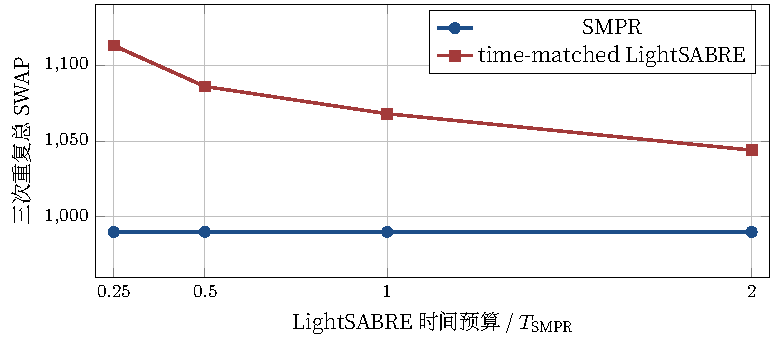
\includegraphics[width=0.80\textwidth]{figures/fig_v7_frontier.pdf}
\caption{LightSABRE 增加时间预算后逐渐缩小与 SMPR 的总 SWAP 差距}
\end{figure}

归一化差值定义为
$({S^{\mathrm{SMPR}}-S^{\mathrm{LS}}})/{M}$。四档预算的公共线路 cluster
bootstrap 95\% 区间依次为
$[-0.359055,0.000724]$、$[-0.319770,0.005950]$、
$[-0.309690,0.015227]$ 和 $[-0.241537,0.023733]$。所有点估计和总量均
有利于 SMPR，且随着 LightSABRE 预算增加，优势从 11.05\% 单调收窄到
5.17\%，形成合理的质量--时间趋势。但区间上端均略大于零，因此不能写成
95\% 水平的统计显著优势。三次重复主要控制同机时间波动；真正的统计簇仍只有
10 条独立公共线路。

\subsection{证据包复算}

V7 证据 ZIP 的 SHA-256 为
\texttt{a8e21b91...8b9a9a75}。包内 29 个文件的总 SHA-256 清单全部通过；
冻结目录、分析目录和三个重复目录的嵌套清单也全部通过。将三份
\texttt{paired\_frontier.csv} 置于独立目录重新运行冻结分析器后，
\texttt{summary.json} 与 \texttt{REPORT.md} 均与上传版本逐字节一致。

\section{复现命令与验收标准}

统一命令行依次执行环境检查、测试、V5/V6 完整路由、统计审计和证据
复算。验收标准如下：

\begin{table}[H]
\centering
\caption{最终验收条件}
\begin{tabularx}{\textwidth}{Y C{2.2cm}}
\toprule
检查 & 要求 \\
\midrule
源发布清单 & 零缺失、零多余、全部哈希一致 \\
公开核心 Python 内置测试 & 20/20 \\
V5 质量参考 & exact 差异为 0 \\
V6 主质量参考 & primary 差异为 0 \\
V5 三项审计 & 60/60/60 \\
V6 三项审计 & 120/120/120 \\
V6 安全质量下界 & 120/120 \\
实例级 bootstrap & 95\% 区间上端小于 0 \\
单元级 bootstrap & 95\% 区间上端小于 0 \\
证据文件哈希 & 18/18 \\
对外来源名称 & 零旧名称泄漏 \\
V7 冻结文件 & 82 个，清单哈希一致 \\
V7 配对观测 & 120/120 \\
V7 环境与重复哈希 & 3/3，3/3 \\
V7 三项审计 & 120/120/120 \\
\bottomrule
\end{tabularx}
\end{table}

\section{最终结论}

冻结 V6 证据、事后稳健性审计和 2026-07-25 独立环境重跑给出一致结论：
SMPR 在显式保留 20-seed LightSABRE 候选的条件下，将总 SWAP 从 3176
降至 3051，减少 3.9358\%，且 120 个实例中没有 SWAP 退化。两个 bootstrap
区间均完全低于零，所有留一层级的总改善仍为正；语义、拓扑和指标审计均为
120/120。

这一证据足以支持冻结构造分布上的安全组合与总体质量改善，但不把组合收益
归因于任何单独内部分支，也不宣称相对单独 LightSABRE 的运行时间优势。
V7 又将实验扩展到 10 条 11--23 比特公共线路和 heavy-hex。四档匹配预算
下，SMPR 的总 SWAP 分别减少 11.05\%、8.84\%、7.30\% 和 5.17\%，
冻结与 120/120 审计完整通过；但四个公共线路 cluster 区间均跨零，故该结果
支持正向外部趋势，不构成 95\% 水平的普遍优势证明。

公开核心已将代码、依赖、测试、冻结配置、V7 规程和发布清单整理为可复核
候选包；完整研发过程和 V7 验证证据分别保存。进一步算法改动应提升版本号，
并使用新的未见数据。

\appendix
\section{最终复算摘要}

% Public paper table reconstructed from the independently verified evidence.
\begin{table}[H]
\centering
\small
\caption{独立环境中的完整质量复现}
\label{tab:independent-reproduction}
\begin{tabular}{lrrrrrr}
\toprule
数据集 & 实例 & LightSABRE & SMPR & 减少 & 墙钟/s & 质量差异 \\
\midrule
V5 & 60 & 1691 & 1641 & 50 & 195.156 & 0 \\
V6 & 120 & 3176 & 3051 & 125 & 527.188 & 0 \\
\bottomrule
\end{tabular}
\end{table}


\begin{notebox}
对外逐实例表中的分支名称是正式名称；原始冻结 CSV 仍保留旧内部字段和值，以
便与既有 SHA-256 证据逐字节核对。论文结论均来自重新计算的数值字段，不依赖
旧控制台文本的字符编码。
\end{notebox}

\end{document}
